\documentclass[a4paper]{article}

%% Language and font encodings
\usepackage[english]{babel}
\usepackage[utf8x]{inputenc}
\usepackage[T1]{fontenc}

%% Sets page size and margins
\usepackage[a4paper,top=3cm,bottom=2cm,left=3cm,right=3cm,marginparwidth=1.75cm]{geometry}

%% Useful packages
\usepackage{amsmath}
\usepackage{graphicx}
\usepackage[colorinlistoftodos]{todonotes}
\usepackage[colorlinks=true, allcolors=blue]{hyperref}

\title{Assignment 4: Design an Implementation of your System (DIS)}
\author{Christa Wright (wrighch3),\\ Kuan-Yu Lai,\\ Blake Hudson(hudsonbl), \\Eric Sisson (sissone), \\ Jorge Guzman Nader(guzmannj)}

\begin{document}
\maketitle
\tableofcontents
\pagebreak

\section{Introduction}

The Zombie Apocalypse Prep App is a web application that allows users to reach their fitness goals in a unique way to train for the zombie apocalypse. The user will create their own goals, and gain points by completing the goals, thus increasing their chances of survival in the event of a zombie apocalypse happening. 

\section{UML Class Diagram}
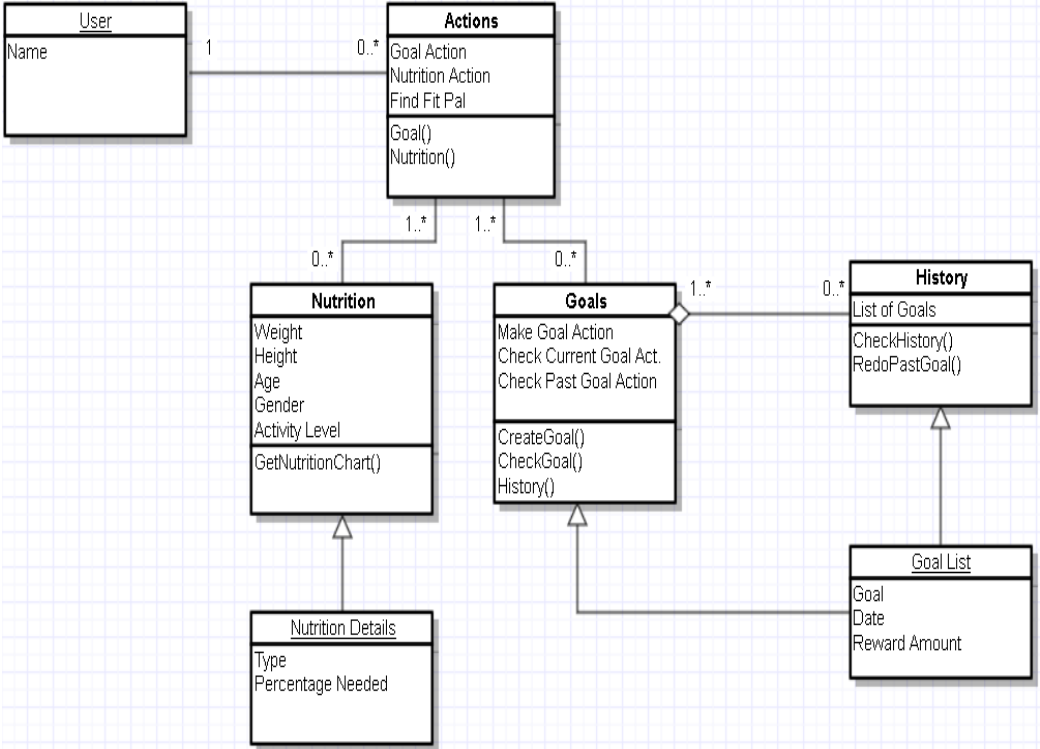
\includegraphics[width=\linewidth]{umldiagram.PNG}

\section{Packages}
Each package is deployed by a web page. Thus, the packages will be tightly coupled because the HTML and CSS format will be similar to each other. The input (tabs from the navigation bar, user input sections, buttons) will only affect packages child elements. The child and parent elements will be explained in each  subsection below.

\subsection{User}
The user affects the content of the page. Thus, the user is loosely coupled with the output of the preceding content of the page. For instance, the user can select Actions, Goals, History and Nutrition. Changing the view of the page. These actions don't actually change the content of those pages or the packages themselves. The user has a strong level of cohesion with the inputs. Inputs consist of setting goals inside of the Goals function. This dynamically prints what the user inputs to the screen after the input is validated.

\subsection{Actions}
The actions package is how the user interacts with the page. Actions are tightly coupled with the output of the page. It's cohesion level is strong because as discussed in the User package, the actions taken on the page changes the content on the page.

\subsection{Goals}
The Goals package only affects: History, and Goal List. The package is loosely coupled with: Nutrition, and Nutrition Details. While being tightly coupled with History, and Goal List. Again the Goals are strongly cohesive with History and Goal List. This is due to the fact that the Goal package is where the user creates and selects input. The input then gets printed and saved in the History and Goal List package.

\subsection{History}
The History package is loosely coupled with every package. Its only function is to print saved input from recent achievements and output from the Goal List. The package is weakly cohesive with itself. The contents within History cannot affect itself. Only other packages can affect the content within History.

\subsection{Goal List}
The Goal List package is loosely coupled with every package except the History package. Once a goal is achieved on the goal list, it is recorded onto the history package. This package is weakly cohesive with the rest of the packages because it does not affect any content on the other pages.

\subsection{Nutrition}
The Nutrition package is loosely coupled with every package. The Nutrition package displays a section where the User package affects the content of the page. The package is strongly cohesive with Nutrition Details. The Nutrition Details package is analogous to the Goal List and Goal package relationship. Where input is selected on this package and sent to another package to print the outcome.

\subsection{Nutrition Details}
The Nutrition Details package is loosely coupled with every package. It is strongly cohesive with the Nutrition package. Because the output of the page grabs input from the Nutrition package. The Nutrition Details package is weakly cohesive with the rest of the packages.

\section{Design Patterns}
The interface of the Zombie Apocalypse Prep App is will consist of a homepage, two pages where the user will input their information, a page where they can review previous goals and a page here their goals will be the main focus. \\

\noindent The web application will emphasize simplicity with minimal constraints, while allowing the options the user has to remain visible. The interface will feature a navigation bar, to allow the user to choose other options, and permit the user to fulfill their goals with great ease. The main constraints the user would have would be not allowing the user to continue entering their nutritional information if they did not enter something within the allowed bounds. This limitation would restrict the user in cases where they are asked to enter their age, but instead they enter a character or word. 
\newline
\newline
\subsection{Consistency}
The web application will follow internal consistency by keeping the navigation bar on all pages, while also allowing the logo to take the user back to the homepage. The input of information will also remain consistent, following most web forms formats. The user will not be able to continue until they have entered information that the program can accept. If the user enters information that the program was not anticipating, then the input text box will turn red, and they will be prompted to enter valid information.\\

\noindent This system follows external consistency of most web forms, consider the sign up information for Facebook, image below [1]. Their input was where 'Apples and oranges' is located, was expecting either an email address, or a phone number, instead an invalid format was inputed and the text box turned read with an exclamation mark. When the exclamation is hovered on, a small popup appears giving the user information. Our web application will not have a pop up, but instead text that directs the user to input correct information.\\

\graphicspath{files/webform.jpg}
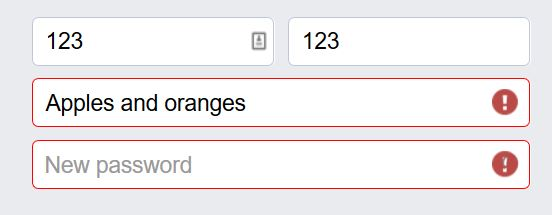
\includegraphics[width = 10cm, height = 5cm]{webform}

\subsection{Shortcuts}
The Zombie Apocalypse Prep app will have some shortcuts the for user. If the user wants to input goals that they have previously inputed, they can review their history and choose that goal again. Or, if they want to make a new goal, they will easily be accomplish this by selecting an activity then input the miles or length of time they want to do this activity. 

\subsection{Informative Feedback}
The user will know that they have accomplished an action, such as inputing nutritional information, or creating a goal by seeing a green success flash banner under the navigation bar. This will offer feedback to the user, along with their information being displayed on the homepage, letting them know they have accomplished their task.

\subsection{Design Dialog Yield Closure}
The system will yield closure of creating a goal by displaying the newly made goals on the homepage with the other goals the user has made. In the event of having completed inputing nutritional information, a chart suggestion nutritional information will be displayed on the homepage. Both of these events will provide feedback with the green flash banner. This is how the user will know the task of inputing information is completed. When a goal is completed, the user will gain points and see their progress bar increase. Additionally, the user will be able to see their completed goals in the history section of the web application.

\subsection{Simple Error Handling}
The opportunity for an error to occur would be upon inputing information to the application. Another error would be if the user accidentally marked that they completed a task without intending to. To prevent the first problem becoming frustrating to the user, helpful text would guide the user along. The visibility of the text would offer guidance to the user, while keeping the data that would cause errors minimal. 

\subsection{Easy Reversal of Actions}
The user will always be able to undo an action. Consider a user submitting incorrect information to the nutritional form. They would easily be able to edit their information to correct it and resubmit the information, allowing them to get correct information. Additionally, if a user enters incorrect information about a goal, they can undo this action by also editing the goal. 

\subsection{Internal Locus of Control}

The user will be in complete control of the web application, and actions will only be initiated if the user has clicked on an action button. Otherwise, the web application will remain stationary, waiting for input.

\subsection{Reduce Short-Term Memory load of Users}

The design of the web application will remain simple, with just a few buttons on each page, with informative text describing what the button will do. Additionally, the links will remain consistent so the user will not have to learn how to navigate each new page.

\section{Interfaces \& Contract}

\subsection{Make Goals}
\textbf{User} The user should be able to easily enter goals according to what they are interested in. The goals will be formatted.
\newline
\newline
\textbf{Engineer} The engineer will create preprogrammed activities that the user could choose from. These activities need to be a physical activity to help the user survive the Zombie Apocalypse, such as running, swimming, or lifting weights. Depending on the activity, the amount of time or distance should be available for the user to choose from. Additionally, the goals will act as in a CRUD format. That is, the user will be able to create, read, update and delete their goals[3]. 

\subsection{Nutrition}
\textbf{User} The user will provide a numerical value of age, height, weight, gender, activity level and the program will output a table with the recommended quantity in mass (grams, milligrams, etc...)that the user must consume daily to be healthy.
\newline
\newline
\textbf{Engineer} The program will accept numerical inputs that will be stored in different variables named age, weight, height and activity level, the variables will be used in metabolic calculations that will provide a table of nutrients with mass quantities in units of grams, milligrams etc. That will show next to the specific nutriment.Some of the daily nutritional requirements will be retrieved form webs nutrition base web pages [2].

\subsection{Error Handling}
\textbf{User} If a user enters invalid information, they can expect text and colored warnings to guide them to correct the information, and continue to complete their task.
\newline
\newline
\textbf{Engineer} The engineer will program a web application to check for strings and integers that are located in the correct section. The user won't be able to continue until this is done. The programmer must write logic that will keep the user from trying to process invalid information.


\section{Exceptions and Handling}
\graphicspath{ {files/Exceptions.png} }
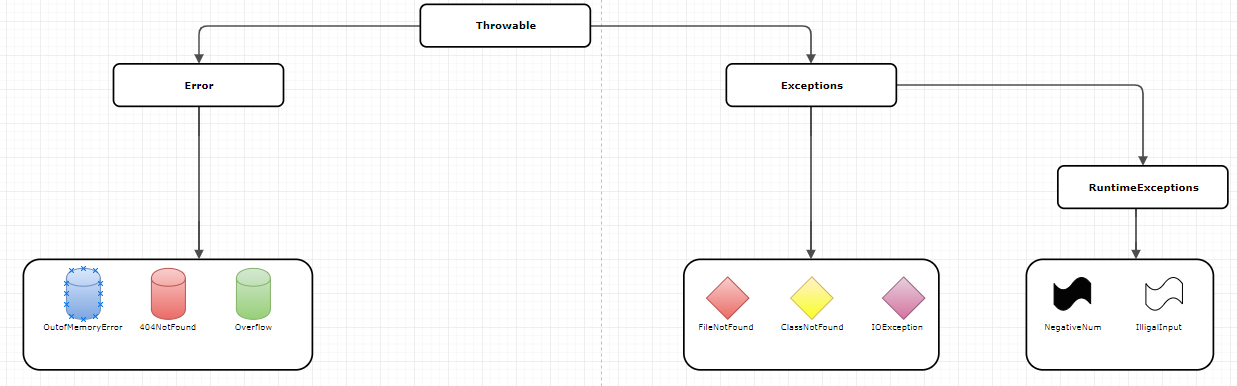
\includegraphics[width = 15cm, height=10cm]{Exceptions}

\noindent Errors that could occur int the program can relate to overflow, 404 page and run out of memory, when such error occur we could display a page to indicate the user that said error had happened.\\

\noindent Some of the most important exceptions that our program will present, are wrong inputs such as negative or out of boundary number, as well as wrong type of input like characters instead of numbers. To handle these exceptions we could prevent the clicking of the output button when wrong input is provided, also a prop message indicating that an error had occur would be shown.\\

\subsection{Meeting report}

\subsection{Progress this week}
This week we start to plan how to handle errors and other sort of problems that can occur in runtime, we also refine the user interface, its functionality and  display, we also plan how we will program the front-end of the project and the objects that it will use .\\
We also map how the objects in the program will interact with each other (coupling and cohesion) and if we can reuse functions or variables to make the code more efficient.

\subsection{Next week plans}
We plan to deploy the first part of the front-end for the project next week. We will focus in implement the user interface based in the models and diagrams that we proposed previously.\\

\noindent We will also organize the oral presentation and decide how we will expose the topics and who will present each topic, based in out familiarity with the topic.\\

\noindent We will also start to make the css/html frame for the project and link the general objects that will be written in JavaScript to the overall frame, important considerations will be put in the dimensions and collection of inputs for the program,wrong handling of this date could have negative effects in how the formulas compute the desires outputs and could slow the development of the whole project. 

\subsection{Member contribution}
We meet Saturday and Sunday and broke the workload in two parts. In Saturday we worked in the UML, the appearance and function of the user interface, how the packages will be organized and used, how our design patters will be, interfaces \& contracts, Which exceptions will be handle and the writing of this report.\\

\noindent Jorge aid in the package section of the assignment, wrote the meeting report and prepared the exceptions diagram, Christa worked in the Design patterns and how they will be implemented and she wrote the interfaces \& Contract section. Blake did the UML class diagram with the help of York, Blake also worked in the package section  and how they relate to the whole project.\\

In Sunday Jorge, York and Eric contributed  in the making of the presentation slides and the overall  brain storming for the project, York also contributed to the diagrams used in the presentations.


\pagebreak
\section{Citations}
[1] https://www.facebook.com
\newline
\newline
[2] https://www.nutrition.org.uk/nutritionscience/nutrients-food-and-ingredients/nutrient-requirements.html?limit=1\&start=2
\newline
\newline
[3]http://propelorm.org/documentation/03-basic-crud.html



\end{document}